% author Dinupa Nawarathne
% email dinupa3@gmail.com
% date 10-11-2022

\documentclass[12pt, xcolor={dvipsnames}, aspectratio = 169]{beamer}

%
% packages
%
\usepackage{graphicx}
\usepackage{amsmath}
\usepackage{hyperref}
\usepackage[absolute,overlay]{textpos}
\usepackage{mathrsfs}
\usepackage[font=tiny]{caption}

%
% customization
%
\mode<presentation>
{
% custom colors
\definecolor{nmsured}{RGB}{137,18,22}
% custom fonts
\usefonttheme{serif}
\setbeamercolor{title}{bg=White,fg=nmsured}
\setbeamercolor{frametitle}{bg=White,fg=nmsured}
\setbeamercolor{section number projected}{bg=nmsured,fg=White}
\setbeamercolor{subsection number projected}{bg=nmsured,fg=White}
\setbeamertemplate{items}{\color{nmsured}$\blacksquare$}
\setbeamertemplate{section in toc}[square]
\setbeamertemplate{subsection in toc}[square]
\setbeamertemplate{footline}[frame number]
\setbeamertemplate{caption}[numbered]
\setbeamerfont{footnote}{size=\tiny}
\setbeamercovered{invisible}
}

%
% title, author, date
%
\title{Vertex Tagging: Sanity Check}

\author{Dinupa}

\date{NMSU Update
\\ October 21, 2022 }


%
% some custom commands
%
\newcommand{\twofig}[5]
{
\begin{frame}{#1}

\begin{textblock}{7.0}(0.5, 1.0)
\begin{figure}
    \centering
    \includegraphics[width=7.0cm]{../imgs/#2.png}
    \caption{#3}
\end{figure}
\end{textblock}

\begin{textblock}{7.0}(8.0, 1.0)
\begin{figure}
    \centering
    \includegraphics[width=7.0cm]{../imgs/#4.png}
    \caption{#5}
\end{figure}
\end{textblock}

\end{frame}
}


%
% predictions
%
\newcommand{\predictions}[4]
{
\begin{frame}

\begin{textblock}{7.0}(0.2, 0.2)
    \begin{figure}
        \centering
        \includegraphics[width=7.0cm]{../imgs/#1}
        \caption{Predicted and test #2.}
    \end{figure}
\end{textblock}

\begin{textblock}{7.0}(8.0, 0.2)
    \begin{figure}
        \centering
        \includegraphics[width=7.0cm]{../imgs/#3}
        \caption{Predicted and test #4.}
    \end{figure}
\end{textblock}

\end{frame}
}

%
% resolution plots
%
\newcommand{\resolution}[1]
{
\begin{frame}

\begin{textblock}{14.0}(0.2, 0.2)
    \begin{figure}
        \centering
        \includegraphics[width=14.0cm]{../imgs/#1.png}
        \caption{$#1$ resolution. (right) $\text{Test data} - \text{ML prediction}$. (left) $\text{Test data} - \text{Reco. data (Legacy method)}$}
    \end{figure}
\end{textblock}

\end{frame}
}

%
% asymmetry check
%
\newcommand{\asymcheck}[2]
{
\begin{frame}

\begin{textblock}{14.0}(0.2, 0.2)
    \begin{figure}
        \centering
        \includegraphics[width=14.0cm]{../imgs/#1.png}
        \caption{asymmetry check for #2. (right) $abs(\text{momentum})$. (left) $\text{positive mom.} - \text{negative mom.}$}
    \end{figure}
\end{textblock}

\end{frame}
}



\begin{document}

% make title page
\begin{frame}
    \maketitle
\end{frame}

\twofig{ROC Curve and Confusion Matrix}
{roc-curve}
{ROC curve for the tagging task.}
{cls-cm}
{Confusion matrix for the tagging task.}

\twofig{Loss}
{cls-loss}
{Loss for tagging task.}
{reg-loss}
{Loss for the regression task.}


\begin{frame}[fragile]{Tagging Task}
    \begin{textblock}{7.0}(0.2, 1.0)
        \begin{figure}
            \centering
            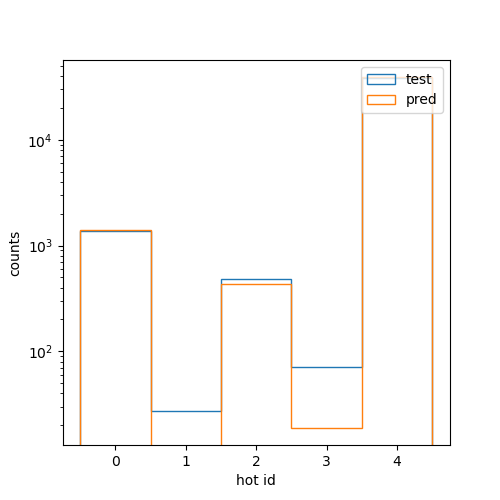
\includegraphics[width=7.0cm]{../imgs/cls-hot-id.png}
            \caption{Predicted and test hot id.}
        \end{figure}
    \end{textblock}
    
    \begin{textblock}{7.0}(7.0, 2.0)
    
    \begin{itemize}
        \item Classification layer almost predict bins except for bin with \verb|hot_id = 1, 3|, with 
        \verb|Accuracy for the test set: 0.9931|
    \end{itemize}
    
    \end{textblock}
    
\end{frame}



\predictions{x [cm].png}{$x$}{y [cm].png}{$y$}
\predictions{z [cm].png}{$z$}{px [GeV].png}{$p_{x}$}
\predictions{py [GeV].png}{$p_{y}$}{pz [GeV].png}{$p_{z}$}


\resolution{x}
\resolution{y}
\resolution{z}
\resolution{px}
\resolution{py}
\resolution{pz}


% \asymcheck{test-px}{$px$}
% \asymcheck{preds-px}{$px$}
% \asymcheck{test-py}{$py$}
% \asymcheck{preds-py}{$py$}

\begin{frame}[fragile]{Asymmetry Check}

\begin{textblock}{7.0}(0.5, 2.0)
    \begin{figure}
        \centering
        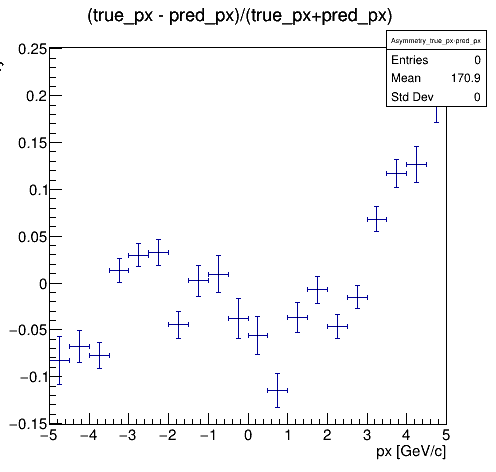
\includegraphics[width=7.0cm]{../imgs/asym-px.png}
        \caption{Asymmetry in $p_{x}$.}
    \end{figure}
\end{textblock}

\begin{textblock}{7.0}(8.0, 2.0)
    \begin{figure}
        \centering
        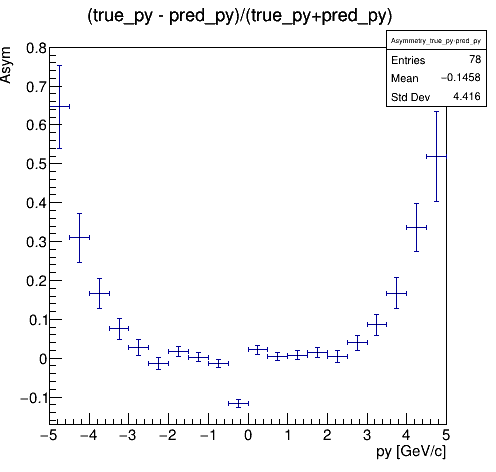
\includegraphics[width=7.0cm]{../imgs/asym-py.png}
        \caption{Asymmetry in $p_{y}$.}
    \end{figure}
\end{textblock}

\begin{textblock}{5.0}(6.0, 0.2)
\color{blue}
\begin{equation*}
\text{Asymmetry} = \frac{\text{true} - \text{pred}}{\text{true} + \text{pred}}
\end{equation*}
\end{textblock}

\begin{textblock}{5.0}(11.0, 0.5)
\color{blue}
\begin{tiny}
Used \verb|GetAsymmetry()| function in \verb|TH1D| in \verb|ROOT|
\end{tiny}
\end{textblock}

\end{frame}


\end{document}